% Options for packages loaded elsewhere
\PassOptionsToPackage{unicode}{hyperref}
\PassOptionsToPackage{hyphens}{url}
\PassOptionsToPackage{dvipsnames,svgnames*,x11names*}{xcolor}
%
\documentclass[
  11pt,
]{book}
\usepackage{amsmath,amssymb}
\usepackage[]{mathpazo}
\usepackage{ifxetex,ifluatex}
\ifnum 0\ifxetex 1\fi\ifluatex 1\fi=0 % if pdftex
  \usepackage[T1]{fontenc}
  \usepackage[utf8]{inputenc}
  \usepackage{textcomp} % provide euro and other symbols
\else % if luatex or xetex
  \usepackage{unicode-math}
  \defaultfontfeatures{Scale=MatchLowercase}
  \defaultfontfeatures[\rmfamily]{Ligatures=TeX,Scale=1}
\fi
% Use upquote if available, for straight quotes in verbatim environments
\IfFileExists{upquote.sty}{\usepackage{upquote}}{}
\IfFileExists{microtype.sty}{% use microtype if available
  \usepackage[]{microtype}
  \UseMicrotypeSet[protrusion]{basicmath} % disable protrusion for tt fonts
}{}
\makeatletter
\@ifundefined{KOMAClassName}{% if non-KOMA class
  \IfFileExists{parskip.sty}{%
    \usepackage{parskip}
  }{% else
    \setlength{\parindent}{0pt}
    \setlength{\parskip}{6pt plus 2pt minus 1pt}}
}{% if KOMA class
  \KOMAoptions{parskip=half}}
\makeatother
\usepackage{xcolor}
\IfFileExists{xurl.sty}{\usepackage{xurl}}{} % add URL line breaks if available
\IfFileExists{bookmark.sty}{\usepackage{bookmark}}{\usepackage{hyperref}}
\hypersetup{
  pdftitle={Data Science Project Guide: Spotify},
  pdfauthor={TechAcademy e.V.},
  colorlinks=true,
  linkcolor=Maroon,
  filecolor=Maroon,
  citecolor=Blue,
  urlcolor=blue,
  pdfcreator={LaTeX via pandoc}}
\urlstyle{same} % disable monospaced font for URLs
\usepackage[top=0.5in, bottom=1.5in, left=1in, right=1in, a4paper]{geometry}
\usepackage{longtable,booktabs,array}
\usepackage{calc} % for calculating minipage widths
% Correct order of tables after \paragraph or \subparagraph
\usepackage{etoolbox}
\makeatletter
\patchcmd\longtable{\par}{\if@noskipsec\mbox{}\fi\par}{}{}
\makeatother
% Allow footnotes in longtable head/foot
\IfFileExists{footnotehyper.sty}{\usepackage{footnotehyper}}{\usepackage{footnote}}
\makesavenoteenv{longtable}
\usepackage{graphicx}
\makeatletter
\def\maxwidth{\ifdim\Gin@nat@width>\linewidth\linewidth\else\Gin@nat@width\fi}
\def\maxheight{\ifdim\Gin@nat@height>\textheight\textheight\else\Gin@nat@height\fi}
\makeatother
% Scale images if necessary, so that they will not overflow the page
% margins by default, and it is still possible to overwrite the defaults
% using explicit options in \includegraphics[width, height, ...]{}
\setkeys{Gin}{width=\maxwidth,height=\maxheight,keepaspectratio}
% Set default figure placement to htbp
\makeatletter
\def\fps@figure{htbp}
\makeatother
\setlength{\emergencystretch}{3em} % prevent overfull lines
\providecommand{\tightlist}{%
  \setlength{\itemsep}{0pt}\setlength{\parskip}{0pt}}
\setcounter{secnumdepth}{5}
\newcommand{\sectionbreak}{\clearpage}
\usepackage{booktabs}
\RequirePackage{fix-cm}
\usepackage[many]{tcolorbox}
\usepackage{xcolor}

\definecolor{r}{HTML}{2369bd}
\definecolor{p}{HTML}{ffde4d}
\definecolor{boxgrey}{HTML}{fefefe}

\newtcolorbox{rbox}{
  colback=boxgrey,
  colframe=r,
  coltext=black,
  boxsep=5pt,
  arc=4pt}
  
\newtcolorbox{pbox}{
  colback=boxgrey,
  colframe=p,
  coltext=black,
  boxsep=5pt,
  arc=4pt}


\newenvironment{tips}[1]
  {
  \begin{itemize}
  \footnotesize
  \renewcommand{\labelitemi}{
    \raisebox{-.7\height}[0pt][0pt]{
      {\setkeys{Gin}{width=3em,keepaspectratio}
        \includegraphics{images/#1.png}}
    }
  }
  \setlength{\fboxsep}{1em}
  \begin{rbox}
  \item
  }
  {
  \end{rbox}
  \end{itemize}
  }
  
  
\newenvironment{tipsp}[1]
  {
  \begin{itemize}
  \footnotesize
  \renewcommand{\labelitemi}{
    \raisebox{-.7\height}[0pt][0pt]{
      {\setkeys{Gin}{width=3em,keepaspectratio}
        \includegraphics{images/#1.png}}
    }
  }
  \setlength{\fboxsep}{1em}
  \begin{pbox}
  \item
  }
  {
  \end{pbox}
  \end{itemize}
  }
  
\usepackage{fancyhdr}
\pagestyle{fancyplain}
\usepackage{setspace}
\usepackage{chngcntr}
\onehalfspacing

\usepackage{titling}
\pretitle{\begin{center}\LARGE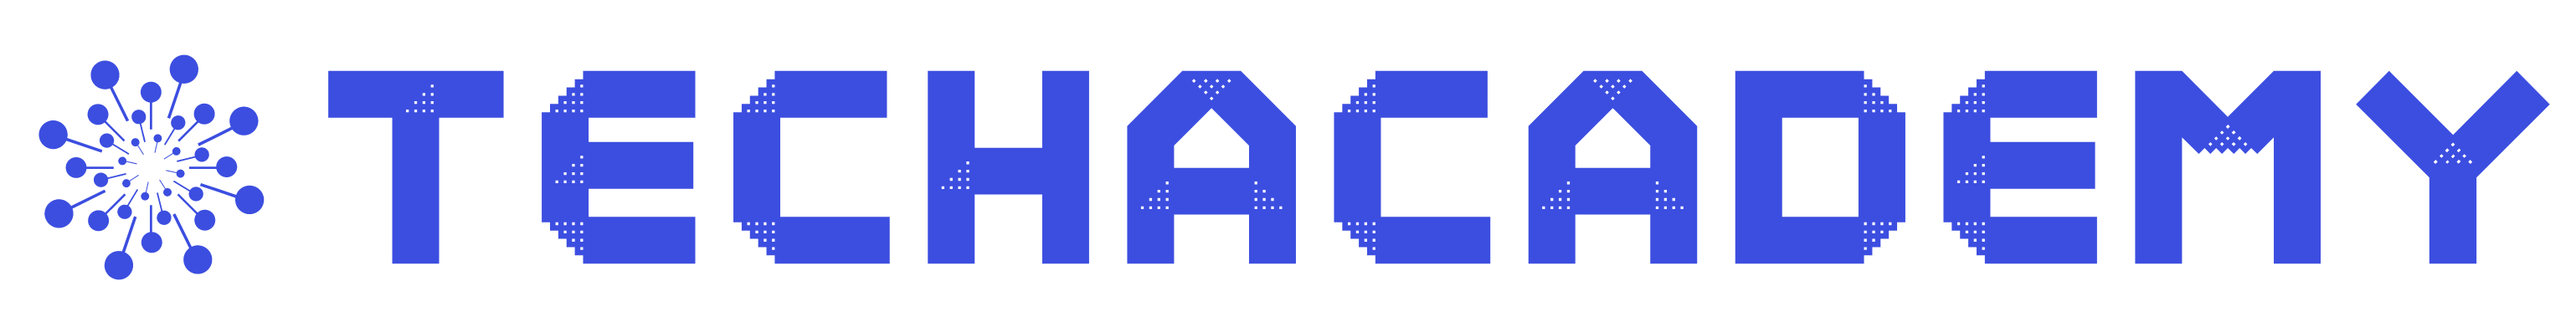
\includegraphics[width=6cm]{plots/TA_Logo.png}\\[\bigskipamount]}
\posttitle{\end{center}}
\ifluatex
  \usepackage{selnolig}  % disable illegal ligatures
\fi
\usepackage[]{natbib}
\bibliographystyle{apalike}

\title{Data Science Project Guide: Spotify}
\author{TechAcademy e.V.}
\date{Summer Term 2021}

\begin{document}
\maketitle

\clearpage

\addtolength{\headheight}{17.82275pt}
\rhead{\includegraphics[height=0.5cm]{plots/TA_logo.png}}

\fancyfoot{}
\fancyfoot[R]{\thepage}
\addtolength{\headheight}{17.82275pt}

\fancyfoot[L]{Data Science Project Guide | Spotify | \copyright\ 2021, TechAcademy e.V.}

\renewcommand{\headrulewidth}{0.25pt}
\renewcommand{\footrulewidth}{0.25pt}

\tableofcontents
\clearpage

\hypertarget{welcome}{%
\chapter{Welcome!}\label{welcome}}

In the first few chapters you will be introduced to the basics of the \texttt{R} and \texttt{Python} tracks respectively and you will find helpful explanations to questions you might have in the beginning of your coding journey. There will be a quick introduction to the Data Science track so that you can get started with the project quickly. So let's get started with the basics!

In all tracks you will work on your project in small groups of fellow students. This not only helps you get the project done faster, it also helps make your results even better. Our experience shows: The different backgrounds of the members and discussing different opinions and ideas will produce the best results. Besides, it is of course more fun to work on a project together than to code alone!\\
The groups can consist of a maximum of four members. You can choose your teammates independently, we won't interfere with your arrangements. It is important that all group members complete the same level of difficulty (beginner or advanced), since the tasks are different in scope for each level. We explicitly encourage you to collaborate with students from different departments. This not only allows you to get to know people from other departments, but may even give you a whole new perspective on the project and tasks.\\
When submitting it is important to note: for a certificate, each person must submit the project individually. However, this can be identical within your group. You can get more information at our first Coding Meetup on \textbf{May 19, 2021}.

This Spotify case study and the associated project guide was developed and written entirely from scratch by TechAcademy's Data Science team. Karlo Lukic and Lara Zaremba developed the project in \texttt{R}, while Felix Schneider and Manuel Mair am Tinkhof developed it in \texttt{Python}.

\hypertarget{whats-data-science-and-how-do-i-do-it}{%
\chapter{What's Data Science and How Do I Do It?}\label{whats-data-science-and-how-do-i-do-it}}

Data science is a multi-layered field in which the use of the latest machine learning methods is only a sub-area. To get there, you'll need many steps before -- from collecting to manipulating to exploring the data. And eventually, you will need to somehow communicate your findings.

But first things first. To analyze data, it must first be obtained. You need to know where to obtain it and how to integrate it in your respective tools. The data is rarely available as it would be needed for further processing. Familiarizing yourself with the information available, cleaning it up and processing it into the desired formats that can be read by humans and machines are important steps that often make up a large part of the work.

Before the obtained data can be analyzed, the right tool must be selected and mastered: the programming language. The most often used languages for Data Science are \texttt{R}, which was explicitly developed for statistics, and \texttt{Python}, which is characterized by its additional versatility. The data scientist does not have to be a perfect software developer who masters every detail and paradigm, but the competent handling of syntax and idiosyncrasies is essential.
There are some well-developed method collections, so-called packages or libraries, which provide a lot of functionality. The use of these collections also has to be learned and mastered.
Once all of this is achieved, the data can finally be analyzed. Here too, it is important to know and understand the multitude of statistical approaches in order to be able to choose the right method for the problem at hand. The newest, best, most beautiful neural network is not always the solution for everything.\\
One step is still missing in the data science process: understanding and communicating the results. The results are often not spontaneously intuitive or sometimes even surprising. Here, the specific expertise and creativity can be played out, especially in the visualization.

\hypertarget{whats-r}{%
\section{What's R?}\label{whats-r}}

\texttt{R} is a programming language that was developed by statisticians in the early 1990s for use in the calculation and visualization of statistical applications. A lot has happened since then and by now, \texttt{R} is one of the most widely used programming languages in the field of data science. Code in \texttt{R} does not have to be compiled, but can be used interactively and dynamically. This makes it possible to quickly gain basic knowledge about existing data and to display it graphically.\\
\texttt{R} offers much more than just programming, but also a complete system for solving statistical problems. A large number of packages and interfaces are available, with which the functionality can be expanded and integration into other applications is made possible.

\hypertarget{rstudio-cloud}{%
\subsection{RStudio Cloud}\label{rstudio-cloud}}

Before you can use \texttt{R}, you usually have to install some separate programs locally on your computer. Typically, you first install a ``raw'' version of \texttt{R}. In theory, you can then already start programming. However, it is very difficult to carry out an entire project with it. That's why there is RStudio, an Integrated Development Environment (IDE) for \texttt{R}. This includes many essential features that simplify programming with \texttt{R}. Among other things, an auto-completion of your code, a nicely structured user interface and many expansion options.

Experience has shown that installing \texttt{R} and RStudio locally takes some effort. Fortunately, RStudio also has a cloud solution that eliminates these steps: RStudio Cloud. There it is possible to edit your project in exactly the same IDE in the browser without any prior installations. You can also easily switch your project from private to public and give your team an insight into your code via a link or by giving them access to the workspace directly. In this way you are able to easily exchange ideas within your team.

We will introduce RStudio Cloud and unlock access to our workspace on our first Coding Meetup. Until then, focus on learning the ``hard skills'' of programming with your courses on DataCamp. This brings us to your curriculum in the next section.

\hypertarget{curriculum}{%
\subsection{Curriculum}\label{curriculum}}

The following list shows the required DataCamp courses for the Data Science with \texttt{R} Track. As a beginner, please stick to the courses of the ``beginner'' program, ambitious beginners can of course also take the advanced courses afterwards. However, the courses should be worked through in the order in which they are listed.\\
The same applies to the advanced courses. Here, too, the specified courses should be processed in the given order. Since it can of course happen that you have already mastered the topics of an advanced course, individual courses can be replaced. The topics of the advanced courses are given in key points. If these key points seem familiar to you, then take a look at the table of contents of the corresponding DataCamp course. If you are convinced that this course does not provide any added value for you, it can be replaced by one of the courses in the ``Exchange Pool'' (see list). However, this exchange course should not be processed until all other courses in the advanced course have been completed.

Both beginners and advanced learners must have completed at least two thirds of the curriculum in order to receive the certificate. For the beginners this means at least up to the course ``Data Visualization with ggplot2 (Part 1)'' and for the advanced at least up to ``Supervised Learning in \texttt{R}: Classification''. In addition, at least two thirds of the project tasks must have been completed.

\begin{tips}r

\textbf{R Fundamentals (Beginner)}

\begin{itemize}
\tightlist
\item
  \href{https://www.datacamp.com/courses/free-introduction-to-r}{Introduction to R (4h)}
\item
  \href{https://www.datacamp.com/courses/intermediate-r}{Intermediate R (6h)}
\item
  \href{https://www.datacamp.com/courses/importing-data-in-r-part-1}{Introduction to Importing Data in R (3h)}
\item
  \href{https://www.datacamp.com/courses/cleaning-data-in-r}{Cleaning Data in R (4h)}
\item
  \href{https://www.datacamp.com/courses/data-manipulation-with-dplyr-in-r}{Data Manipulation with dplyr (4h)}
\item
  \href{https://www.datacamp.com/courses/data-visualization-with-ggplot2-1}{Data Visualization with ggplot2 (Part1) (5h)}
\item
  \href{https://www.datacamp.com/courses/exploratory-data-analysis}{Exploratory Data Analysis in R (4h)}
\item
  \href{https://www.datacamp.com/courses/correlation-and-regression}{Correlation and Regression in R (4h)}
\item
  \href{https://www.datacamp.com/courses/multiple-and-logistic-regression}{Multiple and Logistic Regression in R (4h)}
\end{itemize}

\textbf{Machine Learning Fundamentals in R (Advanced)}

\begin{itemize}
\tightlist
\item
  \href{https://www.datacamp.com/courses/intermediate-r}{Intermediate R (6h)}: conditionals, loops, functions, apply
\item
  \href{https://www.datacamp.com/courses/importing-data-in-r-part-1}{Introduction to Importing Data in R (3h)}: utils, readr, data.table, XLConnect
\item
  \href{https://www.datacamp.com/courses/cleaning-data-in-r}{Cleaning Data in R (4h)}: raw data, tidying \& preparing data
\item
  \href{https://www.datacamp.com/courses/importing-cleaning-data-in-r-case-studies}{Importing \& Cleaning Data in R: Case Studies (4h)}: case studies
\item
  \href{https://www.datacamp.com/courses/data-visualization-with-ggplot2-1}{Data Visualization with ggplot2 (Part1) (5h)}: aesthetics, geometries, qplot
\item
  \href{https://www.datacamp.com/courses/supervised-learning-in-r-classification}{Supervised Learning in R: Classification (4h)}: kNN, naive bayes, logistic regression, classification trees
\item
  \href{https://www.datacamp.com/courses/supervised-learning-in-r-regression}{Supervised learning in R: Regression (4h)}: linear \& non-linear regression, tree-based methods
\item
  \href{https://www.datacamp.com/courses/unsupervised-learning-in-r}{Unsupervised Learning in R (4h)}: k-means, clustering, dimensionality reduction
\item
  \href{https://www.datacamp.com/courses/machine-learning-toolbox}{Machine Learning with caret in R (4h)}: train()-function, cross-validation, auc
\end{itemize}

\textbf{Data Science R (Advanced) -- Exchange Pool}

\begin{itemize}
\tightlist
\item
  \href{https://www.datacamp.com/courses/data-visualization-with-ggplot2-2}{Data Visualization with ggplot2 (Part 2) (5h)}
\item
  \href{https://www.datacamp.com/courses/interactive-maps-with-leaflet-in-r}{Interactive Maps with leaflet in R (4h)}
\item
  \href{https://www.datacamp.com/courses/machine-learning-in-the-tidyverse}{Machine Learning in Tidyverse (5h)}
\item
  \href{https://www.datacamp.com/courses/writing-efficient-r-code}{Writing Efficient R Code (4h)}
\item
  \href{https://www.datacamp.com/courses/support-vector-machines-in-r}{Support Vector Machines in R (4h)}
\item
  \href{https://www.datacamp.com/courses/supervised-learning-in-r-case-studies}{Supervised Learning in R: Case Studies (4h)}
\item
  \href{https://www.datacamp.com/courses/optimizing-r-code-with-rcpp}{Optimizing R Code with Rcpp (4h)}
\end{itemize}

\end{tips}

\hypertarget{links}{%
\subsection{Links}\label{links}}

\begin{itemize}
\tightlist
\item
  RStudio Cheat Sheets: \url{https://rstudio.cloud/learn/cheat-sheets}
\item
  RMarkdown Explanation (to document your analyses): \url{https://rmarkdown.rstudio.com/lesson-1.html}
\item
  StackOverflow (forum for all kinds of coding questions): \url{https://stackoverflow.com/}
\item
  CrossValidated (Statistics and Data Science forum): \url{https://stats.stackexchange.com/}
\end{itemize}

\hypertarget{whats-python}{%
\section{What's Python?}\label{whats-python}}

\texttt{Python} is a dynamic programming language. The code is executed in the interpreter, which means that the code does not first have to be compiled. This makes \texttt{Python} very easy and quick to use. The good usability, easy readability and simple structuring were and still are core ideas in the development of this programming language.
Basically, you can use \texttt{Python} to program according to any paradigm, whereby structured and object-oriented programming is easiest due to the structure of the language, but functional or aspect-oriented programming is also possible. These options give users great freedom to design projects the way they want, but also great freedom to write code that is difficult to understand and confusing. For this reason, certain standards that are based on the so-called \texttt{Python} Enhancement Proposals (PEP) have developed over the decades.

\hypertarget{anaconda-and-jupyter}{%
\subsection{Anaconda and Jupyter}\label{anaconda-and-jupyter}}

Before you can use \texttt{Python}, it must be installed on the computer. \texttt{Python} is already installed on Linux and Unix systems (such as macOS), but often it is an older version. Since there are differences in the handling of \texttt{Python} version 2 -- which is not longer supported anymore -- and version 3, we decided to work with version 3.6 or higher.

One of the easiest ways to get both \texttt{Python} and most of the best known programming libraries is to install Anaconda. There are detailed explanations for the installation on all operating systems on the \href{https://docs.anaconda.com/anaconda/install/}{website} of the provider.

With Anaconda installed, all you have to do is open the Anaconda Navigator and you're ready to go. There are two ways to get started: Spyder or Jupyter. Spyder is the integrated development environment (IDE) for \texttt{Python} and offers all possibilities from syntax highlighting to debugging (links to tutorials below). The other option is to use Jupyter or Jupyter notebooks. It is an internet technology based interface for executing commands. The big advantage of this is that you can quickly write short code pieces and try them out interactively without writing an entire executable program.
Now you can get started! If you have not worked with Jupyter before, we recommend that you complete the course on DataCamp (\url{https://www.datacamp.com/projects/33}) first. There you will get to know many tips and tricks that will make your workflow with Jupyter much easier.

In order to make your work and, above all, the collaboration easier, we are working with the Google Colab platform that contains a Jupyter environment with the necessary libraries. You can then import all the data necessary for the project with Google Drive. We will introduce this environment during our first Coding Meetup. Until then, focus on learning the ``hard skills'' of programming with your courses on DataCamp. This brings us to your curriculum in the next section.

\hypertarget{curriculum-1}{%
\subsection{Curriculum}\label{curriculum-1}}

The following list shows the DataCamp courses for the \texttt{Python} data science track. As a beginner, please follow the courses for the beginner level. These should be processed in the order in which they are listed.\\
The same applies to the advanced courses. Here, too, the specified courses should be processed in the given order. Since it can of course happen that you have already mastered the topics of an advanced course, individual courses can be replaced. The topics of the advanced courses are given in brief. If these key points seem familiar to you, then take a look at the table of contents of the corresponding DataCamp course.
If you are convinced that this course does not provide any added value for you, it can be replaced by one of the courses in the ``Exchange Pool'' (see list). However, this course should not be processed until all other courses in the intermediate \texttt{Python} course have been completed.

Both beginners and advanced learners must have completed at least two thirds of the curriculum in order to receive the certificate. For beginners this means at least up to the course \href{https://learn.datacamp.com/courses/merging-dataframes-with-pandas}{Merging DataFrames with pandas (4h)} (including this course) and for advanced learners at least up to the \href{https://learn.datacamp.com/courses/exploratory-data-analysis-in-python}{Exploratory Data Analysis in Phyton (4h)} (including this course). In addition, at least two thirds of the project tasks have to be completed.

\begin{tipsp}p

\textbf{Python Fundamentals (Beginner) }

\begin{itemize}
\tightlist
\item
  \href{https://www.datacamp.com/courses/introduction-to-data-science-in-python}{Introduction to Data Science in Python (4h)}
\item
  \href{https://www.datacamp.com/courses/intermediate-python-for-data-science}{Intermediate Python (4h)}
\item
  \href{https://www.datacamp.com/courses/python-data-science-toolbox-part-1}{Python for Data Science Toolbox (Part 1) (3h)}
\item
  \href{https://www.datacamp.com/courses/introduction-to-matplotlib}{Introduction to Data Visualization with Matplotlib (4h)}
\item
  \href{https://www.datacamp.com/courses/manipulating-dataframes-with-pandas}{Manipulating DataFrames with pandas (4h)}
\item
  \href{https://www.datacamp.com/courses/merging-dataframes-with-pandas}{Merging DataFrames with pandas (4h)}
\item
  \href{https://www.datacamp.com/courses/exploratory-data-analysis-in-python}{Exploratory Data Analysis in Phyton (4h)}
\item
  \href{https://www.datacamp.com/projects/33}{Introduction to DataCamp Projects (2h)}
\item
  \href{https://www.datacamp.com/courses/introduction-to-linear-modeling-in-python}{Introduction to Linear Modeling in Python (4h)}
\end{itemize}

\textbf{Data Science with Python (Advanced) }

\begin{itemize}
\tightlist
\item
  \href{https://www.datacamp.com/courses/intermediate-python-for-data-science}{Intermediate Python (4h)}: Matplotlib, Dict, Pandas, Loops
\item
  \href{https://www.datacamp.com/courses/python-data-science-toolbox-part-1}{Python Data Science Toolbox (Part 1) (3h)}: Default arguments, Lambdas, Error handling
\item
  \href{https://www.datacamp.com/courses/python-data-science-toolbox-part-2}{Python Data Science Toolbox (Part 2) (4h)}: Iterators, generators, List comprehension
\item
  \href{https://www.datacamp.com/courses/cleaning-data-in-python}{Cleaning Data in Python (4h)}: Using pandas for Data cleaning
\item
  \href{https://www.datacamp.com/projects/82}{Exploring the Bitcoin Cryptocurrency Market (3h)}: Small project
\item
  \href{https://www.datacamp.com/courses/exploratory-data-analysis-in-python}{Exploratory Data Analysis in Phyton (4h)}: How to start a data analysis
\item
  \href{https://www.datacamp.com/courses/introduction-to-linear-modeling-in-python}{Introduction to Linear Modeling in Python (4h)}: Linear Regression, sklearn
\item
  \href{https://www.datacamp.com/courses/supervised-learning-with-scikit-learn}{Supervised Learning with Scikit-Learn (4h)}: Classification, Regression, Tuning
\item
  \href{https://www.datacamp.com/courses/linear-classifiers-in-python}{Linear Classifiers in Python (4h)}: Logistic regression, SVM, Loss functions
\end{itemize}

\textbf{Data Science with Python (Advanced) - Exchange Pool}

\begin{itemize}
\tightlist
\item
  \href{https://www.datacamp.com/projects/684}{TV, Halftime Shows and the Big Game (4h)}
\item
  \href{https://www.datacamp.com/courses/interactive-data-visualization-with-bokeh}{Interactive Data Visualization with Bokeh (4h)}
\item
  \href{https://www.datacamp.com/courses/introduction-to-time-series-analysis-in-python}{Time Series Analysis (4h)}
\item
  \href{https://www.datacamp.com/courses/machine-learning-for-time-series-data-in-python}{Machine Learning for Time Series Data in Python (4h)}
\item
  \href{https://www.datacamp.com/courses/advanced-deep-learning-with-keras-in-python}{Advanced Deep Learning with Keras (4h)}
\item
  \href{https://www.datacamp.com/courses/data-visualization-with-seaborn}{Data Visualization with Seaborn (4h)}
\item
  \href{https://www.datacamp.com/courses/web-scraping-with-python}{Web Scraping in Python (4h)}
\item
  \href{https://www.datacamp.com/courses/writing-efficient-python-code}{Writing Efficient Python Code (4h)}
\item
  \href{https://www.datacamp.com/courses/unsupervised-learning-in-python}{Unsupervised Learning in Python (4h)}
\item
  \href{https://www.datacamp.com/courses/optimizing-python-code-with-pandas}{Writing Efficient Code with pandas (4h)}
\item
  \href{https://www.datacamp.com/courses/deep-learning-in-python}{Introduction to Deep Learning in Python (4h)}
\item
  \href{https://www.datacamp.com/courses/forecasting-using-arima-models-in-python}{ARIMA Models in Python (4h)}
\end{itemize}

\end{tipsp}

\hypertarget{links-1}{%
\subsection{Links}\label{links-1}}

Official Tutorials/Documentation:

\begin{itemize}
\tightlist
\item
  \url{https://docs.python.org/3/tutorial/index.html}
\item
  \url{https://jupyter.org/documentation}
\end{itemize}

Further Explanations:

\begin{itemize}
\tightlist
\item
  \url{https://pythonprogramming.net/}
\item
  \url{https://automatetheboringstuff.com/}
\item
  \url{https://www.reddit.com/r/learnpython}
\item
  \url{https://www.datacamp.com/community/tutorials/tutorial-jupyter-notebook}
\end{itemize}

\hypertarget{your-data-science-project}{%
\section{Your Data Science Project}\label{your-data-science-project}}

\hypertarget{coding-meetups-and-requirements}{%
\subsection{Coding Meetups and Requirements}\label{coding-meetups-and-requirements}}

Now that you have learned the theoretical foundation in the DataCamp courses, you can put your skills into practice. We have put together a project for you based on real data sets. You can read about the details in the following chapters of this project guide.\\
Of course, we will also go into more detail about the project and the tools that go with it. We will discuss everything you need to know during the first Coding Meetup, which will take place on \textbf{May 19, 2021}. After that, the work on the project will officially begin.
You can find the exact project tasks together with further explanations and hints in the following chapters.

To receive the certificate, it is essential that you have solved at least two thirds of the ``Exploratory Data Analysis'' part of the project. For the advanced participants, the entire ``Price Prediction -- The Application of Statistical Models'' part is added. In addition, two thirds of the respective curriculum on DataCamp must be completed. You can find more detailed information on this in the ``Curriculum'' section of the respective programming language above.

\newpage

\hypertarget{introduction-to-your-project}{%
\chapter{Introduction to Your Project}\label{introduction-to-your-project}}

\hypertarget{purpose-of-the-project-guide}{%
\section{Purpose of the Project Guide}\label{purpose-of-the-project-guide}}

Welcome to the project guide for your TechAcademy Data Science project! This document will guide you through the different steps of your project and will provide you with useful hints along the way. However, it is not a detailed step by step manual, because we felt like it was important that you develop the skills of coming up with your own way of solving different tasks. This is a great way to apply the knowledge and tools you have acquired through DataCamp.

It might happen that questions come up or that you don't know how to solve a task right away---but don't worry---this is just part of coding. In those cases you can also find helpful links in the introductory chapters, where your questions might already have been answered. If not, and in the unlikely case that even Google can't help you, the TechAcademy mentors will help you via Slack or directly during the coding meetups.

\textbf{At the end of the project guide you will find an overview of all tasks that have to be completed}, depending on your track (beginner/advanced). You can use this list to check which tasks still need to be completed and which tasks are relevant for your track.

\hypertarget{what-is-this-project-about}{%
\section{What is this Project About?}\label{what-is-this-project-about}}

Last semester, we dealt with the business model of Airbnb. This semester, we will have a look at Spotify data! More precisely, we are first analyzing a very detailed Spotify data set, after which you will get the chance to look at your own Spotify data. You will find all kinds of information in the data sets - useful and useless ones.

Are you already curious to see for yourself? In analogy to the typical Data Science workflow, we split this project into two parts. First you are going to learn how to perform an Exploratory Data Analysis (EDA). You will have a closer look at the data, transform it and then get to know the different variables and what they look like in different types of visualizations. Beginners will have completed the project after this, but it will be beneficial to also try and work on the next part: In the second part of the project you will come up with a model that predicts a song's popularity as accurately as possible. You are going to start with a linear regression model, which you can modify as you please and then you can explore all the other possibilities of modeling and predicting data.

But first things first: What exactly is EDA and what can you achieve with it?

\hypertarget{exploratory-data-analysis-getting-to-know-the-data-set}{%
\section{Exploratory Data Analysis -- getting to know the data set}\label{exploratory-data-analysis-getting-to-know-the-data-set}}

As a first step you will get to know the data set. This means you will describe the data and answer questions like ``Which variables are contained in the data set? \ldots and how are they related?''. For this you can often use graphical tools like box plots or histograms.

This first part of the project is structured in a way that lets you get to know the data thoroughly by completing the given tasks one after the other. As a beginner, you can stop after this part, because you will have fulfilled the necessary coding requirements for the certificate. However, if this first part inspires you to learn more, we encourage you to also work on the second part.

This project guide is structured in the following format. Since the concept of Data Science is independent of specific programming languages, we will describe the general approach in this part of the text. After you understood the overall concept and the tasks we are asking you to do, you will find language-specific tips and tricks in visually separated boxes. If you participate in our \texttt{R}-program, you'll only need to look at the boxes with the blue border. Conversely, you only need to look at the yellow-bordered boxes if you are coding in \texttt{Python}. From time to time it might be interesting to check out the other language -- though you can do the same in both, they sometimes have a different approach to the identical problem. It makes sense that you complete the first few beginner chapters mentioned in the introductory chapter. We recommend that you finish the courses at least until and including \emph{Exploratory Data Analysis} for both tracks.

\hypertarget{prediction-apply-statistical-methods}{%
\section{Prediction -- Apply Statistical Methods}\label{prediction-apply-statistical-methods}}

This part is mainly for the advanced TechAcademy participants. If you are a beginner and you were able to complete the first part without too many difficulties, we highly recommend trying to do the second part as well. Statistical models are a major part of data science and this is your chance of developing skills in this area.

You got to know the data in the first part and you should be familiar with it so that it is now possible to use it to make predictions about a song's popularity based on information you have about the songs in the data set.

For this part of the project, we recommend the advanced courses mentioned in the introductory chapter. Please note that there are more courses available so if you want to extend your skills even further, feel free and complete more courses on the topics that interest you. We recommend that you finish the courses at least until and including \emph{Unsupervised Learning in Python} for the \texttt{Python} track and \emph{Machine Learning Toolbox} for the \texttt{R} track.

Ready? After getting a first impression of what this project is all about, let's get started!

\newpage

\hypertarget{exploratory-data-analysis}{%
\chapter{Exploratory Data Analysis}\label{exploratory-data-analysis}}

At the end of this chapter, you will look into your personal Spotify streaming history. You need to request this data from Spotify, and this can take a few days. Therefore, you should ask for your data as early as possible. Then, start with the first exercises of this chapter which will use some of the data we provide.

\textbf{Download your personal Spotify data}

If you do not use Spotify personally, you can skip this step and start with chapter 4.1.
In chapter 4.5, we will use the requested personal Spotify data, and you can use the data from one of your team members. If nobody on your team uses Spotify, we will provide you with some dummy data.

We will follow eight steps based on \href{https://www.makeuseof.com/tag/download-privacy-data-spotify/}{this} blog post by Dan Price to download your personal Spotify data:
1. Go to \url{https://accounts.spotify.com/en/status} and enter your login credentials.
2. In the menu on the screen's left-hand side, click on Privacy settings.
3. Scroll down to the Download your data section. You will see the following:

\begin{center}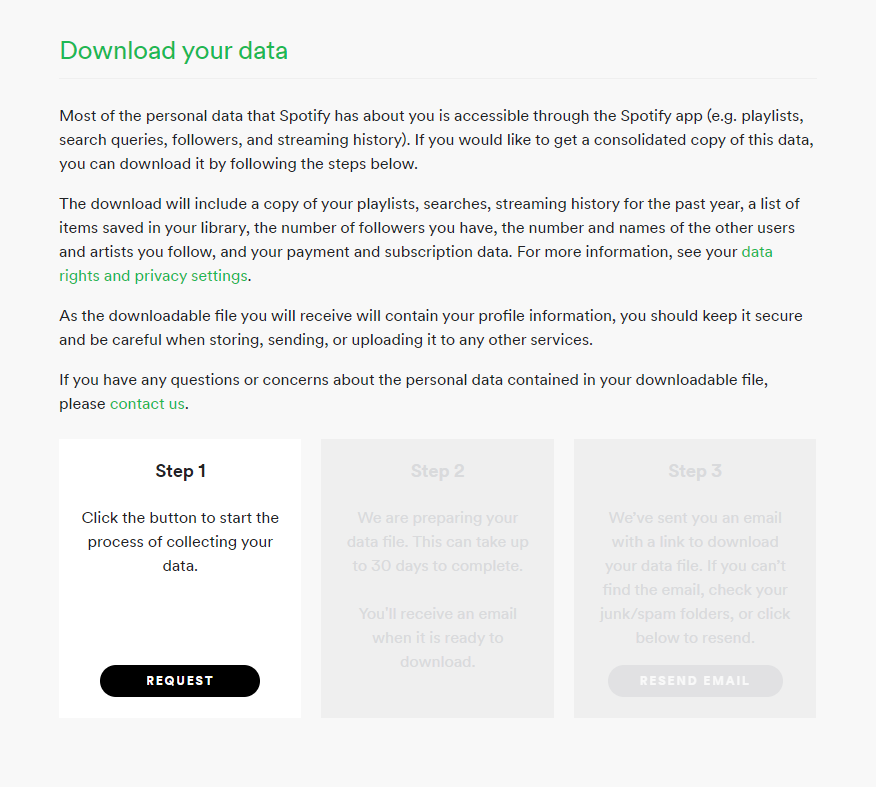
\includegraphics[width=1\linewidth]{splots/spotify} \end{center}

\begin{enumerate}
\def\labelenumi{\arabic{enumi}.}
\setcounter{enumi}{3}
\tightlist
\item
  Click on \emph{Request}. You will probably have to complete a captcha and will receive a confirmation email.
\item
  Click ``Confirm'' in the email. This confirmation will take you back to Spotify, where you will receive an on-screen notification saying:``We are preparing your data file. This {[}process{]} can take up to 30 days to complete. You'll receive an email when it is ready to download.'' - Spotify
\item
  When the data preparation is complete, return to Privacy settings; you will now have access to Step 3.
\item
  Click on Download.
\end{enumerate}

In the next couple of days, you will receive an email from Spotify to download your personal Spotify data as a \texttt{my\_spotify\_data.zip} file. Unzip the file and look for the \texttt{StreamingHistory0.json} file.

\textbf{Hint}: Check what Spotify knows about you by inspecting \texttt{Userdata.json}, \texttt{SearchQueries.json}, or \texttt{Inferences.json} files using Notepad (Windows), TextEdit (MacOS), or VIM (Linux). Surprised? :)

\hypertarget{getting-started}{%
\section{Getting Started}\label{getting-started}}

In this chapter, you will apply the knowledge that you gained throughout the semester to real-world data. The exercises will cover typical problems that you usually encounter when analyzing data.

Before you can dive into the data, set up your programming environment. This will be the place where the magic happens -- all your coding will take place there.

\begin{tips}r

In your workspace on \href{https://rstudio.cloud/projects}{rstudio.cloud}, we have already uploaded an ``assignment'' for you (Template Spotify). When you create a new project within the workspace \emph{Class of '21 \textbar{} TechAcademy \textbar{} Data Science with R}, your workspace will open up. We've already made some arrangements for you: The data sets you will be working with throughout the project are already available in your working directory. We also created an `RMarkdown' file, with which you will be able to create a detailed report of your project. You can convert this file into a PDF document when you have completed the documentation. Open the file ``Markdown\_Spotify.Rmd'' and see for yourself!

\end{tips}

\begin{tipsp}p

We recommend using \href{https://colab.research.google.com}{Google Colab} for this project since it requires no particular setup, stores its notebooks to your Google Drive, and makes it easy for you to share them with your team members.

As an alternative to Google Colab, you might want to install Jupyter Notebook locally using the Anaconda distribution.
Either way, when importing Spotify data, you can use the links to the respective data files provided in the ``Data-Links'' document, which you will find in the TechAcademy drive.

We will give you a more detailed step by step demo during the first coding meetup.

\end{tipsp}

\hypertarget{importing-data}{%
\subsection{Importing Data}\label{importing-data}}

First things first, you will need to load the following two CSV files into your coding environment:

\begin{itemize}
\tightlist
\item
  \href{https://drive.google.com/uc?export=download\&id=1OmFrdUaPFatpPLRikLJHS-VoF1F27G73}{spotify\_songs.csv}
\item
  \href{https://drive.google.com/uc?export=download\&id=1gHO566_qxBbz7t8fcH10uVQDAmxK33IF}{song\_features.csv}
\end{itemize}

How is the data structured, and which variables does it contain? To get a peek at the data you'll be working with, output the first/last few rows.Also, compute some basic descriptive statistics (count, mean, and standard deviation) and determine the column's data types.

\begin{tips}r

First, the data set has to be loaded from your folder structure into the workspace. Import both the \texttt{song\_features.csv} and the \texttt{spotify\_songs.csv} data sets into your workspace (e.g., using \{base\} R's \texttt{read.csv()}, \href{https://readr.tidyverse.org}{\{readr\}}'s \texttt{read\_csv()} or \href{https://rdatatable.gitlab.io/data.table/}{\{data.table\}}'s \texttt{fread()} function) and name the object(s) accordingly.

Though you can name the object however you wish, we recommend using \texttt{original\_file\_name} + e.g., \texttt{\_df} (for data.frame) / \texttt{\_tbl}(for tibble) / \texttt{\_DT} (for data.table) naming convention, so that you can easily distinguish your R objects (data frames, plots, vectors, etc.) later on.

Now, get an overview of the data set. Are there any variables you could drop while reading the data set? You can use the following functions to print the data frame, for example \texttt{head()} or \texttt{glimpse()}.

Lastly, get a quick summary of the data using \{base\} R's \texttt{summary()} or \href{https://personality-project.org/r/psych/}{\{psych\}}'s \texttt{describe()} function.
To find more ways to generate quick data summaries in R, check \href{https://dabblingwithdata.wordpress.com/2018/01/02/my-favourite-r-package-for-summarising-data/}{this} blog post from Adam Medcalf.

\end{tips}

\begin{tipsp}p

Start by importing the pandas' library: \texttt{import\ pandas\ as\ pd}.
You can use the same panda's method you used to import CSV data from your local machine to import CSV data from a web server: Just replace the file path with the URL of the CSV file.

The URLs are:

\begin{itemize}
\tightlist
\item
  spotify\_songs.csv: \url{https://tinyurl.com/TechAcademy-songs}
\item
  song\_features.csv: \url{https://tinyurl.com/TechAcadey-song-features}
\end{itemize}

Finally, get familiar with the data by outputting some of the data frame (e.g.~\texttt{df.head()}), as well as some basic information such as column data types and some descriptive statistics (\texttt{df.info()} \texttt{df.describe()}).

\end{tipsp}

\hypertarget{convert-milliseconds-to-minutes}{%
\subsection{Convert Milliseconds to Minutes}\label{convert-milliseconds-to-minutes}}

\textbf{We will start with the data set ``spotify\_songs.csv''.}

You might have noticed a column with song durations given in milliseconds from the task before. Since (presumably) no one measures song durations in milliseconds, convert them into minutes.

\begin{tips}r

You could use \href{https://dplyr.tidyverse.org/index.html}{\{dplyr\}}'s \texttt{mutate} function to compute and add a new column \texttt{duration\_min} using the existing column \texttt{duration\_ms}. If you haven't heard of the \{dplyr\} package yet, take the respective \href{https://www.datacamp.com/courses/data-manipulation-with-dplyr}{DataCamp course} and the DataCamp's course on \href{https://www.datacamp.com/courses/exploratory-data-analysis}{Exploratory Data Analysis}. Use the respective function and add the new variable to your existing data set.

You can use \href{https://www.timecalculator.net/milliseconds-to-minutes}{this} online calculator as a point of reference for the needed \texttt{mutate()} calculation.

\end{tips}

\begin{tipsp}p

Compute the length of songs in minutes based on the column ``duration\_ms'' and assign it to a new column with

\texttt{df{[}“duration\_minutes”{]}=\ ...}

\end{tipsp}

\hypertarget{song-durations}{%
\subsection{Song Durations}\label{song-durations}}

Next, we want to focus on the concept of distribution:
In this task, you should focus on computing the mean and standard deviation of the duration in minutes and finding the song with the longest duration.
Ideally, the output should be well formatted to something like ``The song with the longest duration is \texttt{{[}song{]}\ by\ {[}artist{]}}.''

\begin{tips}r

Simply use \{base\} R's \texttt{mean()} function to compute a mean of any column in R. Similarly, R comes with \texttt{sd()} function to calculate the standard deviation of a column. You can combine these two functions, e.g., in a \{dplyr\}'s \texttt{summarise()} verb.

Next, find the song with the longest duration (in minutes) using the newly created \texttt{duration\_min} column. The \texttt{filter()} verb from \{dplyr\} in combination with \texttt{max()} function could be helpful in this case. Moreover, you can combine \{dplyr\}'s \texttt{select()} verb with the mentioned \texttt{filter()} verb to show: song's duration, its artist(s) and its name.

For example:

\begin{longtable}[]{@{}rrr@{}}
\toprule
duration\_min & artist(s) & song name \\
\midrule
\endhead
X.X & YY & ZZ \\
\bottomrule
\end{longtable}

\end{tips}

\begin{tipsp}p

Calculating mean and standard deviation should be reasonably easy by applying the mean() and std() function to the corresponding column.

To find the song with the longest duration, you can use pandas \texttt{nlargest} function. You can apply it to a data frame df with \texttt{df.nlargest(n,\ column)}, where n is the number of rows to keep and \texttt{column} defines in which column you want to find the largest values.

\end{tipsp}

\hypertarget{visualizing-song-distributions}{%
\subsection{Visualizing Song Distributions}\label{visualizing-song-distributions}}

Visualizing data is essential to facilitate perception and understanding of information: Create a graph to visualize the distribution of song lengths.

We focus on creating a histogram in the tips section since it's perhaps the most common approach for plotting distributions. You can, however, choose a different chart type; just make sure that the information you want to display is clear and correct.
However, as in school, always add axis labels when possible.

\begin{tips}r

You can use \{base\} R's \texttt{hist()} function to generate a simple histogram of song duration (in minutes). However, we encourage you to use the more extensive \href{https://ggplot2.tidyverse.org}{\{ggplot2\}} package. \{ggplot2\}'s syntax is perhaps a bit harder to learn at the start, but it gives you more plotting benefits over the long run. If you haven't heard of the \{ggplot2\} package yet, take the respective \href{https://www.datacamp.com/courses/data-visualization-with-ggplot2-1}{DataCamp course}.

You could, e.g.~install \href{https://github.com/dreamRs/esquisse\#esquisse-}{\{esquisse\}} package to learn the \{ggplot2\}'s syntax easier. \{esquisse\} will provide you a graphical user interface (GUI) inside RStudio to generate \{ggplot2\} figures. You can then copy/paste the syntax that generated the \{ggplot2\} figure to your R Markdown file. Awesome, eh?

\end{tips}

\begin{tipsp}p

With matplotlibs' \texttt{pyplot.hist(...)}, you can plot a histogram in one line of code.

With some more lines of code, you could (and should) add axis labels.
Try adding a title to the histogram, change the color to your preferences, etc.
Maybe you could even delete outliers with methods such as \texttt{col1.between()} and \texttt{col1.quantile()} - but don't bother with details early on and leave them to the end in case you have enough time.

\end{tipsp}

\begin{center}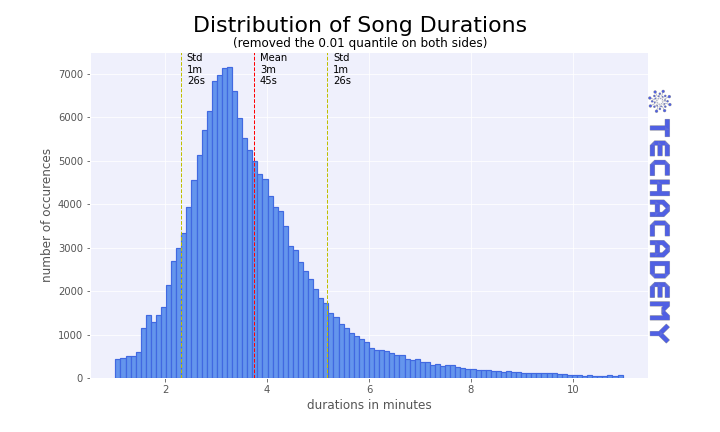
\includegraphics[width=1\linewidth]{splots/durations (3)} \end{center}

\hypertarget{time-series-data}{%
\section{Time Series Data}\label{time-series-data}}

\hypertarget{visualizing-song-durations-over-time}{%
\subsection{Visualizing Song Durations over Time}\label{visualizing-song-durations-over-time}}

While at the topic of song durations, it might also be interesting to see how the average song length evolved: Choose and plot the chart you think is most appropriate for displaying this type of information.

After plotting, please comment/interpret the graph: Were there any significant increases/decreases in song length over time? If so, what could be the reason?

\begin{tips}r

You first need to prepare the data before visualizing it. Generate the average duration of a song (in minutes) by each year. You already used \texttt{summarise()} and \texttt{mean()} functions before. Now, you need to generate that same statistic for each year. You can, e.g., use \{dplyr\}'s \texttt{group\_by()} verb for this purpose.

Afterward, use \{ggplot2\} or \{base\} R's \texttt{plot()} to create a chart.

Please answer open questions in RMarkdown outside the code chunk.

\end{tips}

\begin{tipsp}p

There is a pandas method to group your data frame by year. In combination with the \texttt{.mean()} method, you can compute the average song length by year in one line of code.

Plot the result with matplotlib.

Please answer open questions in text cells.

\end{tipsp}

\begin{center}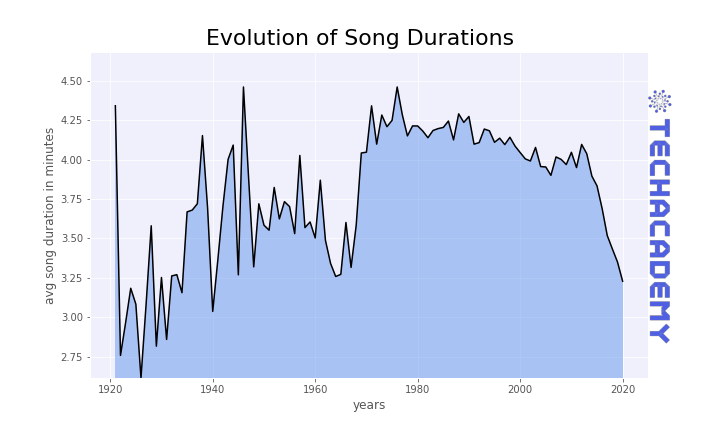
\includegraphics[width=1\linewidth]{splots/durations_over_time} \end{center}

\hypertarget{merge}{%
\subsection{Merge}\label{merge}}

As a data scientist, you'll often find yourself working with data sets from different data sources referencing the same object. For example, you might have the song names in one file and the respective song features in a separate file. It would make more sense to just merge the two data sets into one.

Indeed, this is what happened with our data. So, to make life easier for the upcoming tasks, you'll now need to merge both data sets.
As you might have noticed, there is one column that both data sets share. Find out which column that is and combine the data sets on that column.

\begin{tips}r

You could, e.g., use \{dplyr\}'s \texttt{left\_join()} to combine the two data sets (\texttt{song\_features.csv} and \texttt{songs.csv}) side-by-side.

Take a look at the \href{https://r4ds.had.co.nz/relational-data.html\#understanding-joins}{``R for Data Science''} book for an illustration of join types.

\end{tips}

\begin{tipsp}p

We want to combine the two data sets \texttt{spotify\_songs.csv} and \texttt{song\_features.csv}.
The official documentation of the Pandas library provides a great guide on how to deal with this stuff:
\url{https://pandas.pydata.org/docs/user_guide/merging.html}

\end{tipsp}

\hypertarget{line-plot}{%
\subsection{Line Plot}\label{line-plot}}

Your goal for this task is to plot how `acousticness', `danceability', `energy', `valence', `speechiness', and `instrumentalness' changed over time.

\begin{tips}r

This task involves three steps: creating a summarized data set, reshaping that data set from wide to long format if you'd like to use \{ggplot2\} and finally -- plotting it.

Use the familiar \texttt{group\_by()} and \texttt{summarise()} \{dplyr\} verbs for the first part of the task. Unlike before, include multiple columns in your data summary. Use the familiar \texttt{mean()} function on each column to summarize the data. Save the resulting data summary as a new object.

Use the \href{https://tidyr.tidyverse.org}{\{tidyr\}}'s \texttt{pivot\_longer()} for the second part of the task. \texttt{pivot\_longer()} allows you to transform derived summarized data set from wide to long format by decreasing the number of columns and increasing the number of rows (a.k.a., ``lengthening'' the data). Such transformation is useful for plotting, e.g., in \{ggplot2\}.

Use the \{ggplot2\} to create a line chart of six variables for this task's final step. Alternatively, use the \{base\} R's \texttt{plot()}.

\end{tips}

\begin{tipsp}p

Once again, group the entries by year, get the mean values for the respective column for all years and use matplotlibs' pyplot for plotting.
Don't forget to add a legend and axis labels to the plot.

\end{tipsp}

\begin{center}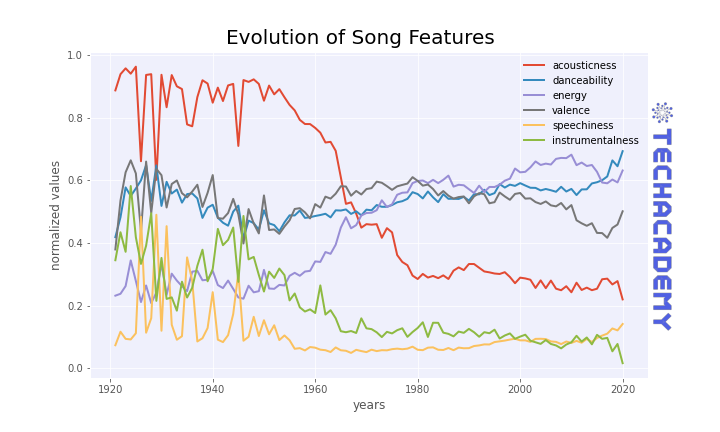
\includegraphics[width=1\linewidth]{splots/features_over_time} \end{center}

\hypertarget{radar-plot-advanced}{%
\subsection{Radar Plot (Advanced)}\label{radar-plot-advanced}}

\textbf{If you are on an advanced track, do this exercise; otherwise, you can skip it.}

Let's get a little fancy by displaying the yearly average song feature values through an interactive radar chart (aka spider plot or polar plot). This chart is very favorable in some cases when you try to display more than two dimensions. Here, each column (or dimension) gets its axis, and the dots on each axis are connected, resulting in a polygon shape.

The features you'll need to plot are: `acousticness', `danceability', `energy', `valence', `speechiness', and `instrumentalness'.

\begin{tips}r

Use the \href{https://plotly.com/r/getting-started/}{\{plotly\}} package to create an interactive Radar/Spider chart of six columns over time. Similar to task 2.3 before, this task will involve summarizing, transforming, and plotting the data.

You are now already experienced in summarizing the data with, e.g., \texttt{group\_by()} and \texttt{summarise()} \{dplyr\} verbs. Focus on summarizing the six columns.

Afterward, transform the data from wide to long format. You could, e.g., use \{tidyr\}'s \texttt{pivot\_longer()} again or \{data.table\}'s \texttt{melt()}.

Lastly, plot the figure using \{plotly\}. Use \href{https://plotly.com/r/radar-chart/}{this} resource as a point of reference for a static plot. Then, create an interactive animation using \href{https://plotly.com/r/animations/}{this} resource.

\end{tips}

\begin{tipsp}p

Here we work with the visualization library plotly, which is a more sophisticated plotting tool than matplotlib:
\texttt{import\ plotly.express\ as\ px}.

Use the already computed data frame with average feature values for each year. Note that after you grouped the data frame, the \texttt{year} column automatically has been set to be the index column -- reverse that (i.e., ``reset'' the index).
Then apply the \texttt{.melt("year")} method on the data frame and have a look at the result. Before continuing, briefly try to understand what happened.

Done that, you can create the radial plot with the \texttt{px.line\_polar(...)} method. The documentation (google something like ``plotly express radar chart'' to find the documentation) tells you which arguments you need (and can) pass to this method:
- Of course, you need to pass some value for the \texttt{data\_frame} argument. For our purpose, this will be the melted data frame.
- You'll also need to pass values for the keyword arguments \texttt{r}, \texttt{theta}, \texttt{animation\_frame}, \texttt{line\_close}, and \texttt{range\_r}.
The values for these arguments are the strings \texttt{“value”}, \texttt{“variable”}, \texttt{“year”}, the boolean value \texttt{True}, and the tuple \texttt{(0,1)} respectively.

Apply \texttt{.show()} directly after the \texttt{line\_polar(...)} method to display the plot.

As always, try updating font size, layout, etc., as you like.

\end{tipsp}

\begin{center}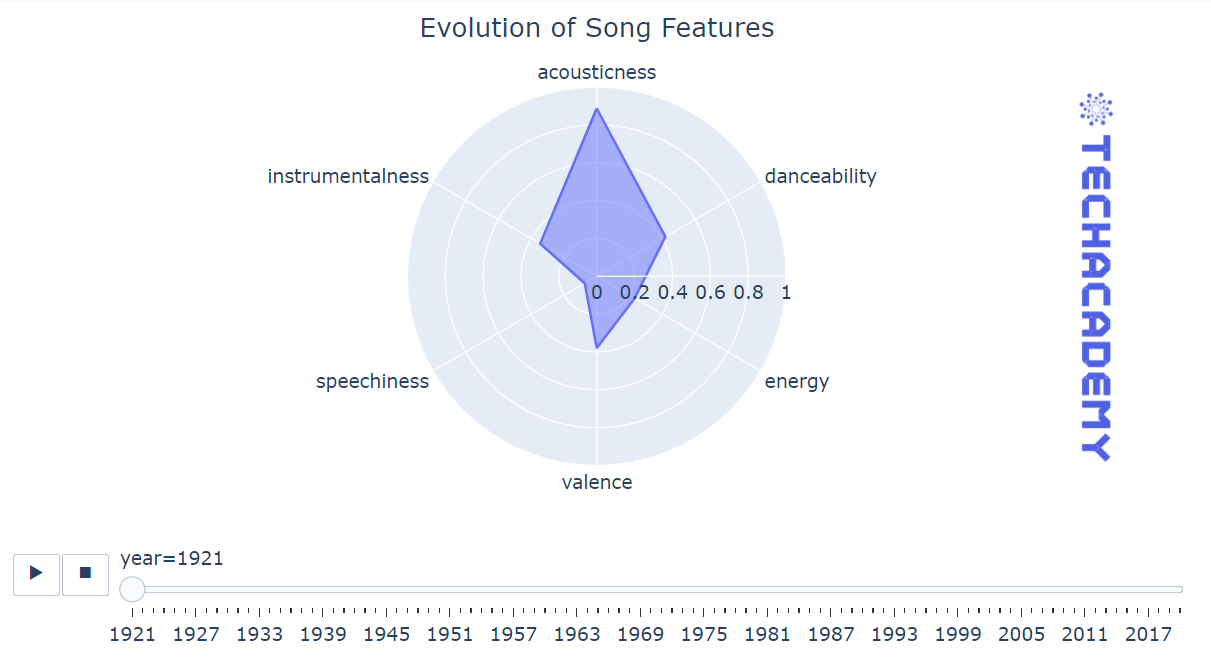
\includegraphics[width=1\linewidth]{splots/features_over_time_advanced} \end{center}

\hypertarget{artists}{%
\section{Artists}\label{artists}}

\hypertarget{most-productive-artists}{%
\subsection{Most Productive Artists}\label{most-productive-artists}}

Our subsequent interest lies in analyzing music artists: Start by showing which artists wrote the most songs using a horizontal bar plot (or any other plot you think works best).

\begin{tips}r

You could use the familiar \texttt{group\_by()} \{dplyr\} verb for this task. However, it would help if you counted the songs of each artist. Does that ring a bell for another \{dplyr\} verb?

After grouping and counting, sort the result by its count. Then, subset the 15 artists with most songs. You can save the derived data summary to a new object.

Lastly, plot the result using \{base\} R or \{ggplot2\} by creating a bar chart.

\end{tips}

\begin{tipsp}p

Pandas' \texttt{.value\_counts(...)} method is all you need to prepare the data.
For plotting use matplotlib's \texttt{plt.barh(...)}.

\end{tipsp}

\begin{center}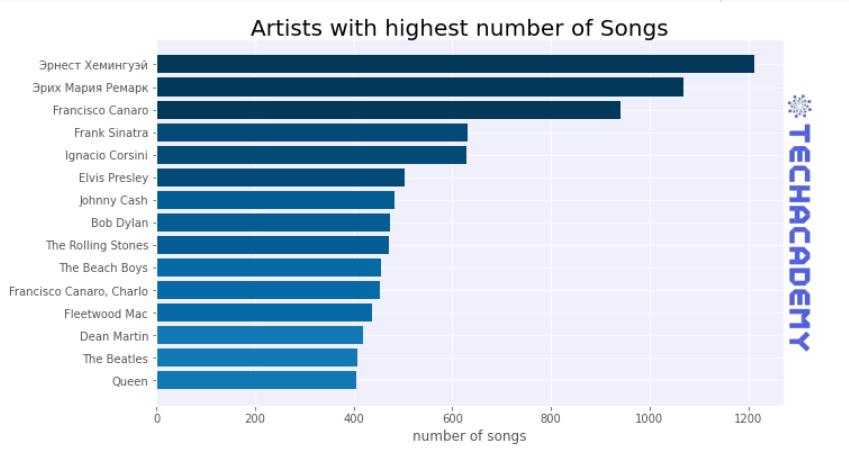
\includegraphics[width=1\linewidth]{splots/artists_bar_chart} \end{center}

\hypertarget{charts}{%
\subsection{Charts}\label{charts}}

Care to discover new songs?

In this section, you'll work with entirely new data (links in the respective tips section).
The goal should be to create a map with a hover effect displaying each country's top song (and its composer) when hovering your mouse over that country.

\begin{tips}r

Use \href{https://jkunst.com/highcharter/}{\{highcharter\}} to create a simple interactive map. Check \href{https://jkunst.com/highcharter/articles/maps.html}{this documentation} if you'd like to do that. In the case of \{highcharter\}, you do not need any additional data as the package relies on \texttt{ISO\ Alpha\ 2} (two-letter) country codes supplied in the data set.

Alternatively, use \{plotly\} to create an interactive map. In this case, you have more customization options, but you need to add \texttt{ISO\ Alpha\ 3} (three-letter) country codes to your data set. You can load \href{https://github.com/lukes/ISO-3166-Countries-with-Regional-Codes/blob/master/all/all.csv}{this CSV file} via URL to merge it with your data set. Then, create a plot using \{plotly\} as described \href{https://plotly.com/r/choropleth-maps/}{here}.

\end{tips}

\begin{tipsp}p

There exists a library for plotting maps: \texttt{import\ folium}.
With folium, you can easily plot a map by running the following two lines:

\begin{verbatim}
m = folium.Map(location=[20,10], zoom_start=2)
m
\end{verbatim}

Folium requires you to specify each country's country border coordinates you like to be drawn (i.e., colored, like in our example map). For this, we prepared a JSON file with all that data. Note that this is not a CSV file; hence you can't use the pandas \texttt{.read\_csv()} method. You'll need to work with two new libraries for importing the data - one for requesting the data from a web server (i.e., Google Drive) and one to parse (i.e., read) the data. Here's the code:

\begin{verbatim}
import requests
import JSON

# request data from a url
response = requests.get(“https://tinyurl.com/TechAcademy-GeoData”)
# parse json data
geo_data = json.loads(response.content)
\end{verbatim}

If you print out the data, you will notice each data subset belongs to a country, and that also contains the top song for the respective country: \texttt{print(geo\_data{[}"features"{]}{[}0{]})\ \ \#\ prints\ data\ of\ the\ first\ country\ in\ JSON\ file}

Now, ``draw'' the country borders by passing the \texttt{geo\_data} as an argument to \texttt{folium.GeoJson(...).add\_to(m)}, and assign it to the variable \texttt{geo}. Note: there is no other variable that needs to be passed as arguments here.
Having done that, add the hover effect displaying each country's top song with \texttt{geo.add\_child(folium.GeoJsonTooltip(...)} and specify fields and aliases through the method's parameters. There is no need to assign this to a variable. You can look up folium's \texttt{GeoJsonTooltip} class online to understand how are fields and aliases passed as arguments.
Display the map by solely typing the letter \texttt{m}.

\end{tipsp}

\begin{center}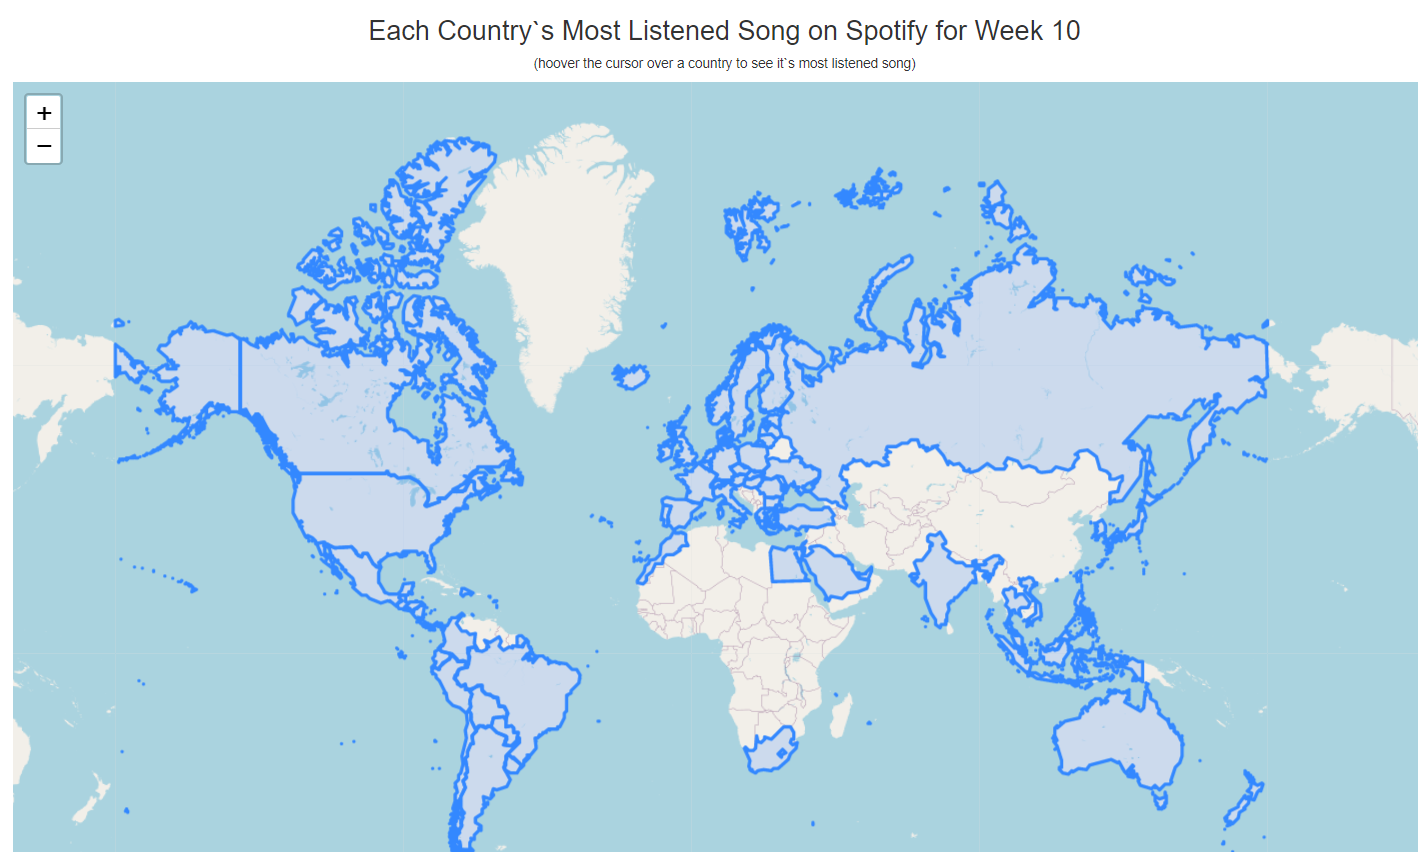
\includegraphics[width=1\linewidth]{splots/map} \end{center}

\hypertarget{compare-artists-based-on-their-songs}{%
\section{Compare Artists Based on their Songs}\label{compare-artists-based-on-their-songs}}

\hypertarget{pairplot-of-different-artists}{%
\subsection{Pairplot of different artists}\label{pairplot-of-different-artists}}

Until now, we analyzed songs individually or compared how many songs individual artists produced. Now, we want to compare the features of songs from artists with each other. For example, how do songs from ``Bob Marley'' differ from ``Nirvana''.
Search in the data set for three different artists or bands which you like. We would recommend that these artists produce music from various genres to see more significant differences between them.

\begin{tips}r

Pick the three artists of your choice (e.g., ``Bob Dylan,'' ``Nirvana,'' and ``Eminem''). You could save your selection to a character vector, e.g., \texttt{my\_artists\_vec}.

You then need to filter/subset the data set for these three artists. That means finding the rows that contain any of those three artists' names. While doing that, make sure to include the four columns of interest for these artists too. You could use \{dplyr\}'s \texttt{filter()} and \texttt{select()} verbs for this purpose.

Afterward, create a pairplot between three artists of your choice. Remember, you are comparing the four features between the three artists. You could use \href{http://ggobi.github.io/ggally/}{\{GGally\}}'s \texttt{ggpairs()} for this purpose. Feel free to play around with the \texttt{ggpairs()} function's arguments as described in \href{http://ggobi.github.io/ggally/articles/ggpairs.html}{its documentation}

\end{tips}

\begin{tipsp}p

Pick three artists of your choice (e.g., ``Bob Dylan'', ``Nirvana'', and ``Eminem''). Filter the data set so that it contains only songs of these three artists.
Now, you can use the \texttt{seaborn} library for visualization. Import this library and use the \texttt{pairplot()} function where you pass the filtered data frame as a parameter, and as the \texttt{hue} value, you choose ``artists''.

\end{tipsp}

\begin{center}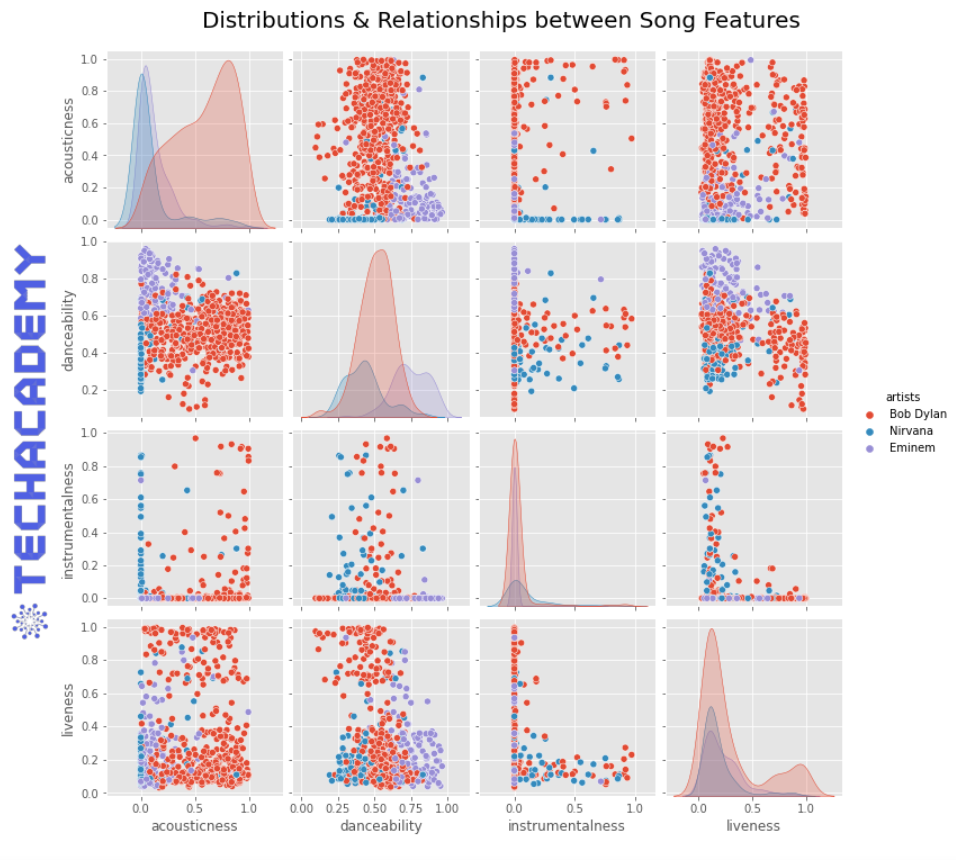
\includegraphics[width=1\linewidth]{splots/feature_comparison} \end{center}

\hypertarget{discover-new-visualization-methods}{%
\subsection{Discover New Visualization Methods}\label{discover-new-visualization-methods}}

Python and R can produce insightful visualizations, and in this exercise, we want to give you an impression of what wide range of visualization types are available. Therefore you can have a look at a gallery that shows a wide range of example plots. Choose one of these possible plots and generate such a plot with the Spotify data.
Write in a comment what your visualization shows and what message it delivers. What insights about the data do you get from this plot?

\begin{tips}r

Visit \href{https://www.r-graph-gallery.com/all-graphs}{``The R Graph Gallery''} to find inspiration for your figure. You could then use either the \{base\} R or the familiar \{ggplot2\} package to create the plot of your choice.

\end{tips}

\begin{tipsp}p

Visit the {[}``Seaborn Gallery''{]} (\url{https://seaborn.pydata.org/examples/index.html\#}), look for a plot that you could use to visualize an aspect of Spotify data and generate a visualization.

\end{tipsp}

\hypertarget{analyse-personal-spotify-data}{%
\section{Analyse Personal Spotify Data}\label{analyse-personal-spotify-data}}

We dived into the provided Spotify data set, and now is the time to look into your personal streaming history. Therefore we use the data set which we requested from Spotify.
If you do not use Spotify, you can also use data from a member of your team. If nobody on your team uses Spotify, contact your mentor, and we will provide you with some dummy data.
Each year Spotify generates a personal wrap-up of your streaming history. Now, we want to produce something similar. First, we want to look at our favorite artists and afterward into our streaming behavior. On which days do we listen to more music or at which times of the day?
This section only scratches the surface of what is possible after you receive your Spotify data. We will illustrate some ideas on how you can analyze your data. In the end, we will mention how you could expand your analysis.

\hypertarget{generate-bar-plot-with-top-10-artists}{%
\subsection{Generate Bar Plot with Top 10 artists}\label{generate-bar-plot-with-top-10-artists}}

We want to start with a Bar plot that shows your favorite artists.
First, we have to load the data into our work environment. If you look at the downloaded data, you can see the \texttt{StreamingHistory0.json} JSON file. This file, however, is not a CSV file. But this is not a big problem as you will see.

\begin{tips}r

First of all, you have to upload your data to access it on RStudio Cloud. Check \href{https://community.rstudio.com/t/importing-data-into-r-studio-cloud/14332/5}{this} series of posts on how to do it. Click on the \texttt{Files} tab in the right pane of your RStudio dashboard. You will then find the \texttt{Upload} button right below the \texttt{Packages} button. After uploading your file, you will see it in your RStudio dashboard under the \texttt{Files} tab -- ready to be loaded.

You can use the \texttt{fromJSON()} function available in \href{https://cran.r-project.org/package=jsonlite}{\{jsonlite\}}, \href{https://cran.r-project.org/package=rjson}{\{rjson\}} or \href{https://cran.r-project.org/package=RJSONIO}{\{RJSONIO\}} package to load the \texttt{StreamingHistory0.json} file into your session. This works similar like, e.g., \texttt{read\_csv()} function that you already used to load a CSV file.

Pick the package whose naming convention comes off most intuitively to you, load the JSON file via \texttt{fromJSON()} and save it as a familiar data frame object (e.g., \texttt{streaming\_history\_df}).

\end{tips}

\begin{tipsp}p

First of all, you have to upload your data to access it with Google Colab. On the left side, you can find a ``Folder'' symbol. Click on it, and you can upload your data with drag and drop. The path to your file is then ``/content/your\_filename.json''.
Until now, we loaded CSV-Files with the pandas method:
\texttt{pd.read\_csv(file)}
So, what pandas method could you use to load JSON files ;) ?

\end{tipsp}

After you loaded the file into your environment, take some time to first look at the data. Print out a couple of rows and look at what columns this data set contains. It could be helpful again to compute a column ``minutesPlayed'' from the column ``msPlayed''.
Afterward, you can create a graph with the artists you listened to the most.

\begin{tips}r

You could add a variable to your personal Spotify data set which counts the number of times you listened to a particular song. Take advantage, e.g., of \{dplyr\}'s \texttt{mutate()} verb. Name the new variable, for example \texttt{n\_times\_song\_played}.

Afterward, you could arrange the data set by the newly created \texttt{n\_times\_song\_played} variable.

Finally, create a chart of the ten most played artists.

\end{tips}

\begin{tipsp}p

Because we want to group the data by the different artists and count how often they appear, the \texttt{df.groupby()} will be helpful again.
Afterward, you need to sort the data and can then visualize it in a plot.

\end{tipsp}

\hypertarget{visualize-your-streaming-behavior}{%
\subsection{Visualize your Streaming Behavior}\label{visualize-your-streaming-behavior}}

We computed and visualized our favorite artists, but when do we listen to music in general? This question is something we want to analyze now. There are different possibilities to explore this question, and we will start by visualizing how many songs you listened to each day with a line plot. Furthermore, you could plot if you listen to more music in the morning, during the day, or in the evening. On which weekday do you listen to more music? More during the week or on the weekend? There are many different ways to explore your data further.

\begin{tips}r

Take advantage of \href{https://lubridate.tidyverse.org}{\{lubridate\}} package for processing dates and times in R. You can easily extract time information (e.g., year, month, day, hour or minute) from the raw \texttt{endTime} column using \{lubridate\}.

Then, add the extracted time information back to the data set, e.g., via the \texttt{mutate()} verb.

You could then add a song counter column to your data set, e.g., \texttt{n\_listened\_songs\_per\_day} using the familiar \{dplyr\} verbs. Make use of the extracted \texttt{day} information from the raw \texttt{endTime} column while grouping and summarizing the data.

Lastly, create a line chart of your data set using \{base\} R's \texttt{plot()} or \{ggplot2\} package.

\end{tips}

\begin{tipsp}p

First of all, we have to tell pandas that the column ``endTime'' is a date. This can be done with the \texttt{pd.to\_datetime()} function.
Afterward, you can group the entries by date with the following command:
\texttt{df.groupby(by=df{[}‘endTime’{]}.dt.date\textasciigrave{}\textasciigrave{}\textasciigrave{}.\ You\ can\ then,\ for\ example,\ count\ how\ many\ songs\ you\ listened\ to\ each\ day\ or\ sum\ up\ the\ amount\ of\ time\ you\ listened\ to\ and\ visualize\ this\ with\ a\ line\ plot.\ With}df{[}`endTime'{]}.dt.date``` the dt you access the DateTime object, and with .date, you group the data by each date which occurs in the data. But it is also possible to group by day or hour instead of date.
Try it out and visualize it in a plot.

\end{tipsp}

\begin{center}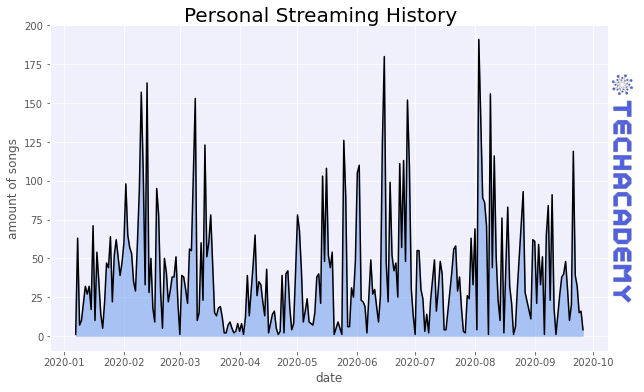
\includegraphics[width=1\linewidth]{splots/personal_streaming} \end{center}

Congratulations -- based on your work with fundamental data transformations and many visualizations, you now have a solid understanding of the Spotify songs data set as well as your personal streaming history. You have now successfully completed the first part of the project! If you are in the beginner group, you have met your minimum requirements. Nevertheless, we strongly recommend that you also have a look at the following part. There you'll be developing methods to predict the popularity of songs! Sounds exciting, doesn't it?

\newpage

\hypertarget{popularity-prediction-application-of-statistical-methods}{%
\chapter{Popularity Prediction -- Application of Statistical Methods}\label{popularity-prediction-application-of-statistical-methods}}

In the previous part you got a feel for the data set. You now know which variables are included and a few characteristic properties of the data set. But so far, we have only visualized the data set. In this section we go a step further and use statistical methods to predict a song's popularity as accurately as possible.

To compare your models, you will use a uniform metric to check the predictions for accuracy. In your case, this is the Root Mean Square Error (RMSE), i.e., the root of the average squared difference between the predicted (\(\hat{y}_i\)) and the actual value (\(y_i\)) :

\[ RMSE = \sqrt{\frac{1}{N}\sum_{i=1}^{N}{(\hat{y}_i-y_i)^2}} \]

The closer the \(RMSE\) is to 0, the better your model predicts prices. Therefore, in the following section, your goal is to reduce the \(RMSE\) of your various models as much as possible through continuous improvements.

We use the Spotify data set, which contains features about the songs as well as their popularity. When we train our model with the data, we need to estimate how well our model predicts popularity values for songs it has never seen before. Therefore we split our data set into two parts - a train and a test set.

Here is a brief description of why you need each data set:

\begin{itemize}
\item
  \emph{train.csv (70 \%)}: You use this training data set to train your model. The model can learn the relationships between the variables based on the training data set containing both the variables needed to predict the popularity and the actual popularity variable.
\item
  \emph{test.csv (30 \%)}: With this test data set, you can test how well your model predicts the popularity using data it has not seen before. This prediction will help you, for example, to recognize under- or overfitting.
\end{itemize}

\begin{tips}r

There are multiple ways to split/partition the data set in R. You could, e.g., use \texttt{createDataPartition()} function from \href{https://cran.r-project.org/package=caret}{\{caret\}}, \texttt{sample.split()} function from \href{https://cran.r-project.org/package=caTools}{\{caTools\}} or --- perhaps most intuitively --- \texttt{split\_train\_test()} function from \href{https://CRAN.R-project.org/package=healthcareai}{\{healthcareai\}}.

Make sure, however, to include the \texttt{set.seed()} function in your R code before randomly dividing the data set into train/test parts. \texttt{set.seed()} function allows you to reproduce randomness each time you re-run your code. That means that you always get the same (random) result -- a vital aspect of reproducibility within the scientific method.

\end{tips}

\begin{tipsp}p

The sklearn library has a function that you can use to split the data set, correspondingly
\texttt{from\ sklearn.model\_selection\ import\ train\_test\_split\ X\_train,\ X\_test,\ y\_train,\ y\_test\ =\ train\_test\_split(df,\ df.popularity,\ test\_size=0.3)}

\end{tipsp}

\hypertarget{examine-the-correlation-between-the-variables-train}{%
\section{Examine the Correlation Between the Variables (train)}\label{examine-the-correlation-between-the-variables-train}}

How are the individual variables related to each other? In other words, to what extent do the variables in the data set correlate with one another? Finding this out is extremely important for deciding which model specification to use later. A good place to start is to create a correlation matrix:

\begin{tips}r

Use the \texttt{cor()} function from the \{base\} R to create a correlation matrix. Select all numerical variables in your data set with the help of \texttt{sapply()} or \{dplyr\}'s \texttt{select()} and create a correlation matrix.

Alternatively, use the \texttt{ggcorrplot()} from the same-name \href{https://cran.r-project.org/package=ggcorrplot}{\{ggcorrplot\}} package.

Check out \href{http://jamesmarquezportfolio.com/correlation_matrices_in_r.html}{this article} by James Marquez if you're curious about other ways to create a correlation plot in R.

\end{tips}

\begin{tipsp}p

You can show the correlations between the features by using the \texttt{.corr()} function on a data frame. You can additionally get a colorized version by using \texttt{df.corr().style.background\_gradient()}

\end{tipsp}

Which of your examined variables correlates most with popularity and which seems to be more independent from popularity? You now have a first impression of which variables could be vital for your model. So let's get to your first song popularity prediction model!

\hypertarget{first-predictions-with-simple-regression-models-train}{%
\section{First Predictions with Simple Regression Models (train)}\label{first-predictions-with-simple-regression-models-train}}

Now you can make use of your statistical knowledge. You will need a method with which you can predict the popularity of a Spotify song.

Have you ever heard of linear regression? Now you can use your statistics skills. First, set up a model with popularity as the dependent variable. In the previous exercise, you examined different variables. Now choose the variable with the highest correlation to popularity and use that as the only independent variable.

For example, your first regression model could look like this:

\[popularity = \beta_0 + \beta_1 \cdot danceability \]

\begin{tips}r

In R, you can implement a simple linear regression with the \texttt{lm()} function. You then get the model summary with the \texttt{summary()} function.

Alternatively, check \href{https://vincentarelbundock.github.io/modelsummary/}{\{modelsummary\}} or \href{https://www.jakeruss.com/cheatsheets/stargazer/}{\{stargazer\}} package to pretty-print the results of your regression model(s).

Define both dependent (y\_train) and independent (X\_train) variables and clean the data if necessary.

\end{tips}

\begin{tipsp}p

For the next step the X\_train values need to be reshaped .values.reshape(-1,1). Note: If you use more than one feature, you don't have to reshape your data.

Import LinearRegression() from sklear.linear\_model and train your model using LinearRegression().fit().

\end{tipsp}

Does your independent variable has a statistically significant impact on popularity? Probably yes, because we selected the variable most correlated with popularity. However, if we stick to this very simplified model, we make a typical mistake: the so-called Omitted Variable Bias (OVB). To put it simply, we neglect (in statistics jargon: ``do not control for'') variables that have a significant influence on the dependent variable. One could suspect that other influencing factors also play an important role in estimating a song's popularity. If we do not include them, the estimate of the effect of, e.g., danceability, is biased and hardly helpful. In our case, this is not a big problem for the time being since we are not interested in causal effects but rather in the best possible prediction. Your statistics professor would almost certainly object to such a model. Nonetheless, with just a single explanatory variable, this model will not necessarily predict the popularity well.

One possible solution is simply to include the omitted variables in the model. That is quite practical as the data set already includes these variables. So let's set up a somewhat more extensive model that includes an additional variable:
\[popularity = \beta_0 + \beta_1 \cdot danceability + \beta_2 \cdot energy\]
Now compare the results of these two models. Does the larger model explain a higher proportion of the variance in popularity? In other words, which model shows the higher value for the \(R^2\) measure?

\begin{tips}r

Use the \texttt{summary()} function of your model to compare the two models. Which model shows a higher value for \(R^2\)? Then you can compare the RMSE between your two models.

\end{tips}

\begin{tipsp}p

You can now compare your two models, therefore compute for each model the \(R^2\) value.

\texttt{import\ sklearn.metrics\ as\ metrics\ \ r2=metrics.r2\_score(y\_true,\ y\_pred)}

\end{tipsp}

\hypertarget{from-training-to-testing-making-predictions}{%
\section{From Training to Testing -- Making Predictions}\label{from-training-to-testing-making-predictions}}

You have now trained your first model with the training data set. But how well does the model handle data it has not seen yet? This out-of-sample testing is a critical test to evaluate the quality of your model.

Did your model only ``memorize'' the existing patterns in the training data set? Then the relationships from the training data set would not be transferable to the test data set. With so-called overfitting, you trained the model too closely to the training data set and therefore received poor predictions for unknown data -- for example, the data in your test set.

On the other hand, underfitting is also a problem: Your model did not sufficiently learn the actual relationships between the data. Thus, it makes poor predictions on the test data set. So it is essential to find a balance between the two problems.

Now the distinction between training and test data sets becomes essential. As a reminder: we use the train data to train a model and the test data to test our model's quality.

To test your model on previously unseen data, you can apply it to the test data set.

\begin{tips}r

Use the predict function for this:

\texttt{predicted\_popularity\ \textless{}-\ predict(your\_saved\_model,\ your\_test\_data\_frame)}

You have now created a vector with all popularity predictions for the test data set. You can now compare this with the actual values for popularity from the test data set.

In order to use a uniform comparison metric, please use the following function to measure your prediction accuracy:

\texttt{\#\ Function\ that\ returns\ Root\ Mean\ Squared\ Error\ while\ ignoring\ NAs\ rmse\ \textless{}-\ function(actual,\ predicted)\ \{\ sqrt(mean((predicted\ -\ actual)\^{}2,\ na.rm\ =\ TRUE))}

After training, import the data from the \texttt{test.csv} file, define both variables \texttt{X\_test} and \texttt{y\_test}, and create a vector with price predictions applying \texttt{predict(X\_test)} on your model. Store your prediction in the variable \texttt{predicted\_popularity}.

\end{tips}

\begin{tipsp}p

Finally, compare your predicted values with the test values:

from sklearn.metrics import mean\_squared\_error
\# Function that returns Root Mean Squared Error while ignoring NaNs
rmse = mean\_squared\_error(y\_test, predicted\_popularity, squared=False)

\end{tipsp}

Now compare both regression models. Does the larger model have better prediction accuracy, i.e., a lower \(RMSE\)? Now you have a benchmark for your more advanced models, which you can beat in the next part.

\hypertarget{apply-advanced-machine-learning-algorithms}{%
\section{Apply Advanced Machine Learning Algorithms}\label{apply-advanced-machine-learning-algorithms}}

Now that you have created and tested an initial prediction using a simple regression model, you can apply more advanced methods. The goal is to get the lowest possible \(RMSE\) when applying the model to the test data set. Look for at least one other algorithm and check whether it gives you a more accurate prediction (expressed as a lower \(RMSE\) ). You can find inspiration for this in the advanced DataCamp courses listed at the beginning of the project guide. There are no limits -- you can refine the regression using specific methods (e.g., LASSO) or set up a random forest model or a neural network. It is usually a good idea to briefly recall the respective algorithm's functionality and consider whether this methodology makes sense with a continuous prediction variable.

You can also get a noticeable gain in predictive power by modifying existing variables or generating new variables from the data set (``feature engineering''). For example, you could create features based on artists. You could count the number of songs each artist produced or the mean popularity of each artist. You could also write a function that computes each artist's mean popularity in the train data set and adds these values to the train data set. Afterward, you can add the same values to the test set, but keep in mind that there can be artists in the test set who are not in the train set. Therefore you could set the values for these artists to the mean popularity of all artists.

Always compare the \(RMSE\) of your advanced models with each other, as well as with the benchmark regression model from before.

Congratulations! You've made it to the end of your TechAcademy Data Science project. After visualizing the data in the first part, you've also set up predictive models in this section. If you stuck around until this part and managed to code the better part of the exercises, you've definitively earned your certificate! We hope you had fun learning Data Science with this data set and that you enjoyed it -- at least the parts where you didn't get stuck forever because of some unexplainable coding error. Don't forget to send your project results to our project submission email address before the deadline.

\newpage

\hypertarget{excercise-checklist}{%
\chapter{Excercise Checklist}\label{excercise-checklist}}

This checklist should help you keeping track of your exercises. Remember that you have to hand in satisfactory solutions to at least two thirds of the exercises. If you're part of the beginner track this refers to two thirds of part A (EDA) only. If you're part of the advanced track, you have to hand in at least two thirds of both individual parts A and B. Hence, you cannot hand in 100 percent of the first part and only 50 percent of the second one. You'll need more than 66\% in each one for a certificate. After all, you're not really that advanced if you only did half of it, right?

\textbf{Part A: Exploratory Data Analysis (Beginners + Advanced)}

\textbf{Data: Kaggle Data}

\begin{enumerate}
\def\labelenumi{\arabic{enumi}.}
\tightlist
\item
  \textbf{Getting Started}
\end{enumerate}

1.1 Read in data, show data, give summary of data (mean, count,\ldots)

1.2 Compute column ``duration\_minutes'' from ``duration\_ms''

1.3 Compute mean/std of duration\_minutes, which song has the longest duration?

1.4 Plot histogram of song durations

\begin{enumerate}
\def\labelenumi{\arabic{enumi}.}
\setcounter{enumi}{1}
\tightlist
\item
  \textbf{Time Series: How did songs change over the years?}
\end{enumerate}

2.1 Streaming leads to shorter songs? Group-By: song duration over years

2.2 Merge songs with song\_features on id

2.3 Compare how features like `acousticness', `danceability', `energy', `instrumentalness' changed over time

2.4 For Advanced: Radial plot over time

\begin{enumerate}
\def\labelenumi{\arabic{enumi}.}
\setcounter{enumi}{2}
\tightlist
\item
  \textbf{Artists}
\end{enumerate}

3.1 Bar Plot with artists with most songs

3.2 Map with top songs in each country

\begin{enumerate}
\def\labelenumi{\arabic{enumi}.}
\setcounter{enumi}{3}
\tightlist
\item
  \textbf{Pairplot: Artist Comparison}
\end{enumerate}

4.1 Look for three different artists and compare the features of the songs with a pairplot

4.2 Look at the proposed galary and look for a plot which could be used to visualize an aspect of the spotfiy data and generate a plot

4.3 What is the message of your plot? What does it show?

\textbf{Data: Personal Spotify Data}

\begin{enumerate}
\def\labelenumi{\arabic{enumi}.}
\setcounter{enumi}{4}
\tightlist
\item
  \textbf{Personal Data}
\end{enumerate}

5.1 Generate Bar Plot with top 10 artists

5.2 Visualize when you listened to music. On which days, to which times?

\textbf{Part B: Popularity Prediction Using Statistical Methods ((motivated) Beginners + Advanced)}

\textbf{Data: Kaggle Data}

\begin{enumerate}
\def\labelenumi{\arabic{enumi}.}
\item
  Create correlation plot between features
\item
  Regression
\end{enumerate}

2.1 Create simple linear model to predict popularity of song

2.2 Improve your model using more features

\begin{enumerate}
\def\labelenumi{\arabic{enumi}.}
\setcounter{enumi}{2}
\item
  Train/ Test your model
\item
  Develop more advanced models
\end{enumerate}

\newpage

\hypertarget{whats-next-in-your-data-science-career}{%
\chapter{What's Next in Your Data Science Career?}\label{whats-next-in-your-data-science-career}}

At the end of your TechAcademy semester, you've successfully coded your way through a whole Data Science project. You liked what you did and would like bring your skills to the next level? Then this section provides you with many useful resources to deepen your knowledge in Data Science in general or Python and R in particular. The first section is useful for every aspiring Data Scientist, while the two following boxes introduce you to some language-specific resources. If you've come across some other useful materials that we didn't mention here, feel free to contact us -- this list is far from complete!

\hypertarget{data-science-in-general}{%
\section{Data Science in General}\label{data-science-in-general}}

\hypertarget{version-control-with-git}{%
\subsection*{\texorpdfstring{Version Control with \href{https://github.com/}{Git}}{Version Control with Git}}\label{version-control-with-git}}

If you're serious about data science, you will need Git. Better learn it early and start enjoying and appreciating it before it's too late and you're pressured into learning it on the fly! Every project you do should be versioned with Git. Regardless if you're working alone or with a big group of developers. Regardless if you write ten lines of code or a really complex program. With Git, you can keep track of all your changes. It's like a Dropbox/Google Drive for developers, but way better. Pro-Tip: Get free GitHub Pro as a Student with the \href{https://education.github.com/pack}{GitHub Student Developer Pack}. Besides all the perks of GitHub Pro, you'll also free access to many other great tools. See the respective tutorials on how to set up your Git workflow.

\hypertarget{advice-for-non-traditional-data-scientists}{%
\subsection*{\texorpdfstring{Advice for \href{https://blog.shotwell.ca/posts/learning_data_science/}{Non-Traditional Data Scientists}}{Advice for Non-Traditional Data Scientists}}\label{advice-for-non-traditional-data-scientists}}

Important advice from Gordon Shotwell, a former lawyer, on what it takes to have a successful data science career coming from a non-computer science background. Extremely encouraging and helpful read on what you should and shouldn't do to reach that goal.

\hypertarget{learn-from-great-data-scientists-on-kaggle}{%
\subsection*{\texorpdfstring{Learn from Great Data Scientists on \href{https://www.kaggle.com/}{Kaggle}}{Learn from Great Data Scientists on Kaggle}}\label{learn-from-great-data-scientists-on-kaggle}}

Kaggle is a platform that hosts data science challenges. The great thing about it is that you can browse through many clever solutions to tricky machine learning tasks. And of course, you can also join the competition and measure your predictions with others. There are plenty of both Python and R notebooks.

\hypertarget{r}{%
\section{R}\label{r}}

\begin{tips}r

\textbf{Install R and RStudio Locally}

RStudio.Cloud is great for getting started with R without having to worry about installing anything locally. Sooner or later you will have to install everything on your own computer. Here's a \href{https://www.datacamp.com/community/tutorials/installing-R-windows-mac-ubuntu}{DataCamp tutorial} on how to do that.

\textbf{Version Control with Git}

RStudio has a nice interface that lets you enjoy the perks of Git without ever having to touch the command line -- sounds great, does it? Learn how to set up the Git \& R workflow with \href{https://happygitwithr.com/}{Happy Git with R}.

\textbf{\href{https://www.r-graph-gallery.com/}{R Graph Gallery}}

Get inspiration to take your plotting to the next level. Includes code to reproduce the plots.

\textbf{Follow the R Master Himself and the R Community}

Hadley Wickham was and continues to be extremely influential on the development of R and its rise to one of the most popular data science languages. He's behind many tools that we taught you in this semester, especially the tidyverse (including great packages such as ggplot2 and dplyr). Follow him \href{https://twitter.com/hadleywickham}{on Twitter} to get great R advice and keep up to speed with everything new to R. Following the many people behind R (not only Hadley) is a great way for acquiring deeper understanding of the language and its developments.

\textbf{Join the \href{https://www.meetup.com/r-frankfurt/}{Campus useR Group in Frankfurt}}

There's a quite active R community in Frankfurt that meets once a month. It's open for students, professors, industry practitioners, journalists, and all people that love to use R. In those meetings, you'll hear about other's work, discuss new developments, and ask questions.

\textbf{Listen to R Podcasts}
Another great way to easily keep up with new developments in the Data Science/R community. Check out
\href{http://nssdeviations.com/}{Not So Standard Deviations} or \href{https://r-podcast.org/}{the R-Podcast}

\end{tips}

\hypertarget{python}{%
\section{Python}\label{python}}

\begin{tipsp}p

\textbf{Install Python Locally}

Until now you've only programmed using JupyterHub on the TechAcademy Server. A next step would be to install Python and Jupyter locally on your computer. This \href{https://docs.anaconda.com/anaconda/install/}{link} contains the necessary information on how to install the software on Windows, iOS or Linux.

\textbf{Choosing the Right Editor}

Using Jupyter is especially useful for short data analyses. But sometimes you want to write longer scripts in Python. In these cases, it is often more convenient to use a code editor instead of Jupyter. \href{https://realpython.com/learning-paths/perfect-your-python-development-setup/}{This tutorial} highlights the positive aspects of such an editor and how to choose the right one for you. Pro Tip: Also check out the other tutorials on \href{https://realpython.com/}{Real Python}.

\textbf{\href{https://python-graph-gallery.com/}{Python Graph Gallery}}

Get inspiration to take your plotting to the next level. Includes code to reproduce the plots.

\textbf{More Advanced Python Concepts}

You know the basic data structures in Python like lists and dictionaries. What are the next steps to improve your knowledge? \href{https://book.pythontips.com/en/latest/index.html}{This website} gives good explanations for slightly more advanced concepts which can be very useful from time to time.

\textbf{A Deeper Understanding}

If you want to get a deeper understanding of the Python programming language and into typical algorithms which are used in the field of Data Science, this \href{https://github.com/ab-anand/py-books/blob/master/Data\%20Science\%20from\%20Scratch-\%20First\%20Principles\%20with\%20Python.pdf}{free book} can be a good starting point.

\textbf{Writing Beautiful Python Code}

``My code doesn't look nice, but it works!''
This might work for yourself, but often you will work on code with other people. But even if you're just coding for yourself it's a good idea to follow the PEP8 style guide. It's a useful convention on how to structure and code in Python. You'll find useful resources for PEP8 \href{https://realpython.com/python-pep8/}{here} and \href{https://www.python.org/dev/peps/pep-0020/\#id2}{here}.

\textbf{Listen to Python Podcasts}

When you don't have time for books you can listen to \href{https://talkpython.fm/home}{Talk Python} or the \href{https://www.pythonpodcast.com}{Python Podcast}.

\end{tipsp}

  \bibliography{book.bib,packages.bib}

\end{document}
